\section{Implementation with a job shop acting simulator}
\begin{frame}{Validation on a factory simulator with job shop like problems}
    Proposition of a new simulation environment for acting problems: GobotSim
    \begin{itemize}
        \item Simpler than RoboCup
        \item Differs from Craft-bots by targeting job shop problems with scheduling and resource management problematics.
    \end{itemize}
\end{frame}

\begin{frame}{GobotSim environment}
\begin{columns}
    \begin{column}{0.4\textwidth}
        \begin{figure}[tp]
            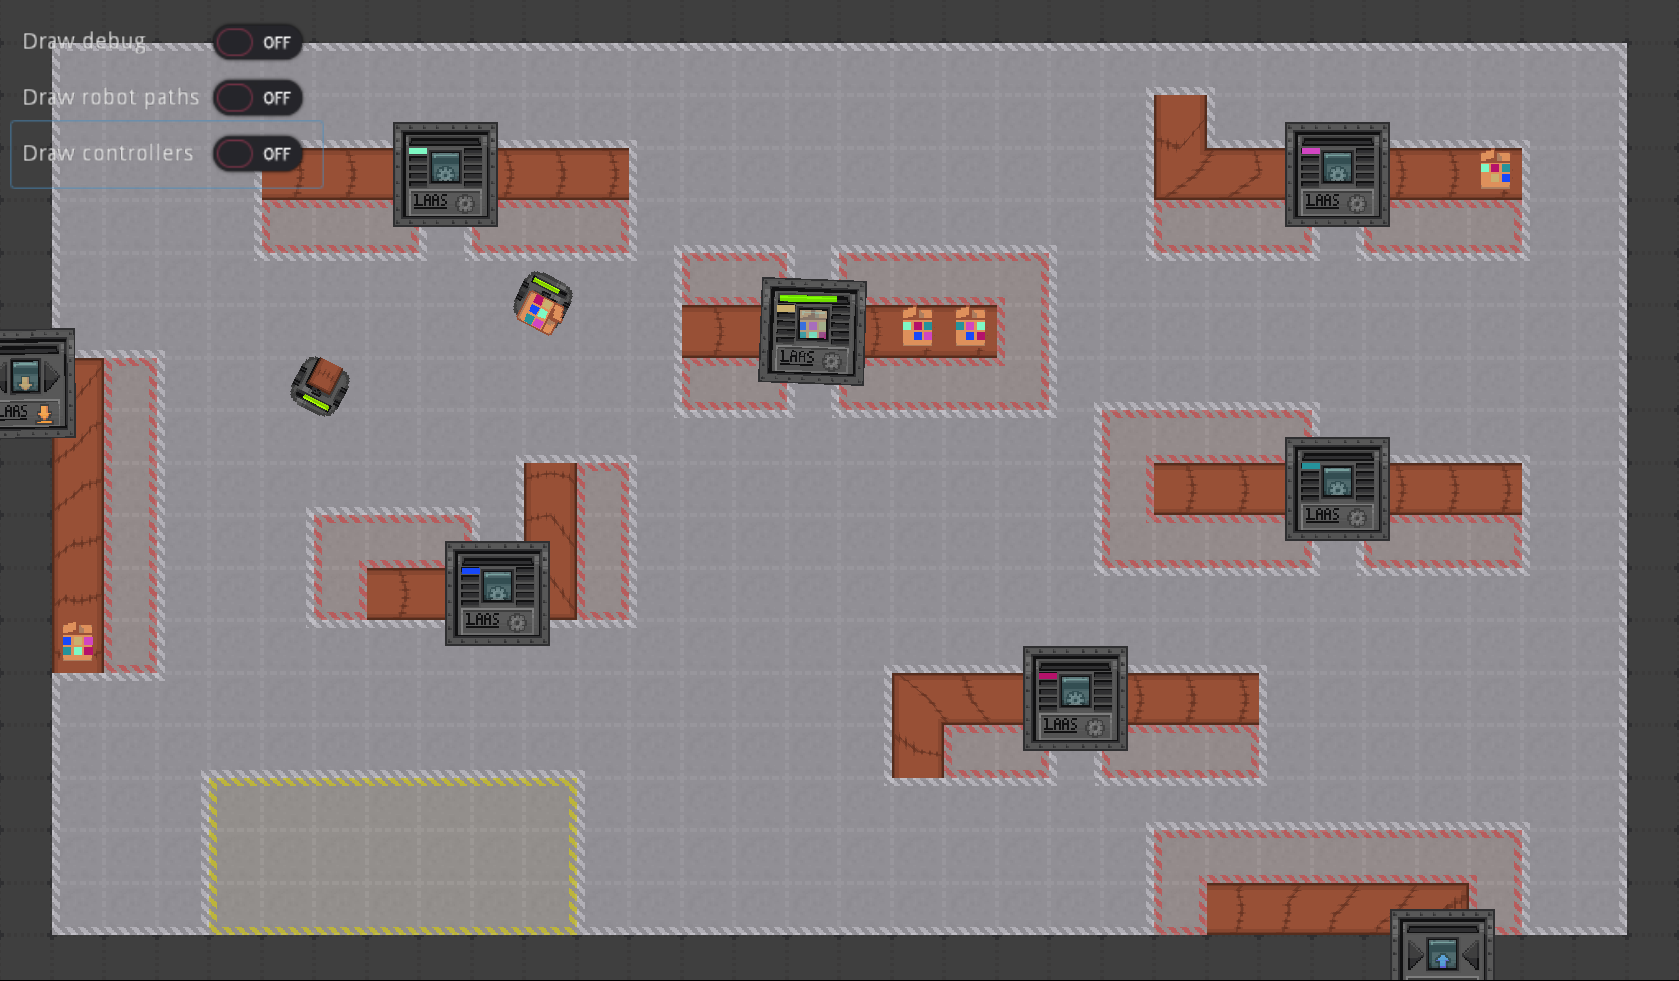
\includegraphics[width=\linewidth]{images/gobot-rae.png}
        \end{figure}
    \end{column}
    \begin{column}{0.5\textwidth}
        Machines
        \begin{itemize}
            \item Processing : does a predefined list of process for packages
            \item Input: generate packages
            \item Output: gather fully processed packages
        \end{itemize}
        Robots : manipulate packages
        \begin{itemize}
            \item commands: move, pick, place,\dots
            \item recharge at recharge areas
        \end{itemize}
    \end{column}
\end{columns}
\end{frame}

\begin{frame}[fragile]{OMPAS models for GobotSim}
    \begin{columns}
        \begin{column}{0.5\textwidth}
            \begin{itemize}
                \item High-level goal: process all packages in the environment
                \item Body of the unique method of the high-level task.
                \setlength{\leftmargini}{0pt}

                \tiny
            \begin{lstlisting}
(do
    (mapf new-resource (instance robot))
    (mapf new-resource (instance machine))
    (define h1 (async (t_process_packages)))
    (define h2 (async (t_check_rob_bat)))
    (await h1))
            \end{lstlisting}    
            \end{itemize}
    

            
        \end{column}
        \begin{column}{0.5\textwidth}
Role of the acting engine : 
\begin{itemize}
    \item Schedule package passage on machines
    \item Allocate package displacement tasks to robots
    \item Monitor the robots' batteries 
\end{itemize} 
    \end{column}
    \end{columns}
    
\end{frame}

\begin{frame}{Validation on Job shop problems}
\centering
%Outline the features of the new system and the language
\begin{columns}
    \begin{column}{0.5\textwidth}
        Restriction of the simulation:
        \begin{itemize}
            \item All packages are created at the beginning
            \item Each machine can do a unique process
        \end{itemize}
    \end{column}
    \begin{column}{0.5\textwidth}
        Different strategies:
        \begin{itemize}
            \item Greedy
            \item Advanced
            \item ALRPTF
        \end{itemize}
    \end{column}
\end{columns}
\end{frame}

\newcommand{\calcrowmean}{
    \def \rowmean{0}
    \pgfmathparse{\pgfkeysvalueof{/pgfplots/table/summary statistics/end index}-\pgfkeysvalueof{/pgfplots/table/summary statistics/start index}+1}
    \edef\numberofcols{\pgfmathresult}
            % ... loop over all columns, summing up the elements
    \pgfplotsforeachungrouped \col in {1,2,3,4,5,6,7,8,9,10}% in {\pgfkeysvalueof{/pgfplots/table/summary statistics/start index},...,\pgfkeysvalueof{/pgfplots/table/summary statistics/end index}}
    {
        
        \typeout{col = \col}
        
        \pgfmathparse{\rowmean+\thisrowno{\col}/\numberofcols}
        \edef \rowmean{\pgfmathresult}
    }
}
\newcommand{\calcstddev}{
    \def\rowstddev{0}
    \calcrowmean
    \pgfplotsforeachungrouped \col in {1,2,3,4,5,6,7,8,9,10}
    % {\pgfkeysvalueof{/pgfplots/table/summary statistics/start index},...,\pgfkeysvalueof{/pgfplots/table/summary statistics/end index}}
    {
        \pgfmathparse{\rowstddev+(\thisrowno{\col}-\rowmean)^2/(\numberofcols-1)}
        \edef\rowstddev{\pgfmathresult}
    }
    \pgfmathparse{sqrt(\rowstddev)}
}
\newcommand{\calcstderror}{
    \calcrowmean
    \calcstddev
    \pgfmathparse{sqrt(\rowstddev)/sqrt(\numberofcols)}
}

\pgfplotstableset{
    summary statistics/start index/.initial=1,
    summary statistics/end index/.initial=10,
    create col/mean/.style={
        /pgfplots/table/create col/assign/.code={% In each row ... 
            \calcrowmean
            \pgfkeyslet{/pgfplots/table/create col/next content}\rowmean
        }
    },
    create col/standard deviation/.style={
        /pgfplots/table/create col/assign/.code={% In each row ... 
            \calcstddev
            \pgfkeyslet{/pgfplots/table/create col/next content}\pgfmathresult
        }
    },
    create col/standard error/.style={
        create col/assign/.code={% In each row ... 
            \calcstderror
            \pgfkeyslet{/pgfplots/table/create col/next content}\pgfmathresult
        }
    }
}

\pgfplotstableset{
    create on use/mean/.style={create col/mean},
    create on use/stddev/.style={create col/standard deviation},
    create on use/stderror/.style={create col/standard error}
}



\begin{frame}{Results comparison}
    \begin{figure}[t]

        \begin{tikzpicture}
          \begin{axis}[
                      /pgf/number format/.cd,
                          use comma,
                      height = 6cm,
                      width = \linewidth,
                      ymajorgrids,
                      ylabel={Time in seconds},
                      xlabel={Problems},
                      ymin = 0,
                      ymax= 220,
                      ybar=0pt,
                      bar width=12pt,
                      enlarge x limits = 0.3,
                      nodes near coords,
                      point meta=explicit symbolic,
                      scatter/position=absolute,
                      every node near coord/.style={
                              at={(\pgfkeysvalueof{/data point/x},1.8)},
                              anchor=south,
                          },
                      bar shift=0pt,
                      xtick={0,1,2,3},
                      xticklabels={p1,p2,p3,p4},
                      x tick label style={rotate=45,anchor=east},
                      legend cell align = {left},
                      legend pos = north west,
                      legend image post style={scale=0.4},
                      legend style={font = \footnotesize},
                  ]
          \addplot+[bar shift = -12pt]
          plot[
                  %smooth,
                  error bars/.cd,
              y dir=both,
              y explicit
          ]
          table[
                  x=Problem,
                  y=mean,
                  y error=stderror
          ]
          {datas/jobshop_greedy.dat};
          \addplot+
          [bar shift = +0pt]
          plot[
                  %smooth,
                  error bars/.cd,
              y dir=both,
              y explicit
          ]
          table[
                  x=Problem,
                  y=mean,
                  y error=stderror
          ]
          {datas/jobshop_advanced.dat};
          \addplot+[bar shift = +12pt]
          plot[
                  %smooth,
                  error bars/.cd,
              y dir=both,
              y explicit
          ]
          table[
                  x=Problem,
                  y=mean,
                  y error=stderror
          ]
          {datas/jobshop_advanced_lrptf.dat};
      
          \legend{
                      Greedy,
                      Advanced,
                      ALRPTF}
        \end{axis}
      \end{tikzpicture}
          \caption{Comparison of the mean time to execute 4 6x6 job-shop problems with three different allocation strategies. Each pair problem-strategy has been executed 10 times.
          Timescale of the simulator is set to 4.}
        \label{fig:gobot-results}
      \end{figure}
\end{frame}